\section{The interval construction and its invariants}\label{sec:construction}

We now construct the hierarchy from a feasible full schedule of \(J\).
Each node has a \emph{tag}, one of the two frames, and a witnessing
complete schedule. Descending to a child changes only the jobs inside
that child; its boundary triples and exterior schedule remain fixed.
Branches can retain separate witnesses, as allowed in
\Cref{def:hierarchy}.

\subsection{Global lists and boundary conditions}

In the tag frame of a node \(W=(a,b)\), attach an ordered list
\(\K=(K_1,\ldots,K_\ell)\) of global upsets.
Define the global qualifier set and the local old-high set by
\[
 \Qual(\K)=\bigcup_{i=1}^{\ell}K_i,
 \qquad O=W\cap\Qual(\K).
\]
For every globally qualifying job \(x\), set
\begin{equation}
 \key_{\K}(x)=
 \left(\max\{i:x\in K_i\},\,\rk(x)\right),
 \label{eq:key}
\end{equation}
with lexicographic comparison. Entries may overlap. Their largest index,
not their smallest one, is used.
Because each entry is an upset, \(x\prec y\) with \(x\) qualifying
implies that \(y\) qualifies and
\(\key_{\K}(x)<\key_{\K}(y)\).

We maintain the following three invariants in the node's tag frame.
\begin{enumerate}[label=\textup{(I\arabic*)},ref=I\arabic*]
 \item\label{inv:cones}
 \(O\subseteq P_b\), and \(W\setminus O\subseteq D_a\).
 \item\label{inv:past}
 Every global qualifier scheduled at or before \(a\) belongs to
 \(\wP a\).
 \item\label{inv:swap}
 After \emph{any} feasible reordering of \(W\) in its existing slots,
 there is no feasible direct exchange between
 \(x\in W\setminus D_a\) and a qualifying job \(y\) at \(a\) when
 \(\key_{\K}(x)<\key_{\K}(y)\).
\end{enumerate}
Invariant~\ref{inv:cones} controls the jobs inside the interval;
Invariant~\ref{inv:past} controls qualifiers outside its left boundary,
and Invariant~\ref{inv:swap} makes that control persist after later
reorderings.

The exchange in Invariant~\ref{inv:swap} is tested for feasibility in
the complete schedule. The hypothetical exchanged schedule need not
preserve any decomposition or any of the list invariants.
The key of \(x\) is defined because Invariant~\ref{inv:cones} implies
\(W\setminus D_a\subseteq O\). A sentinel has no boundary jobs, so
the corresponding exchange condition is vacuous.

Lexicographic minimality within an interval controls exchanges of its
interior jobs; it gives no such control over exchanges with an exterior
boundary job. Invariant~\ref{inv:swap} supplies the latter control.
Suppose a qualifying job \(x\in W\setminus D_a\) has all its
predecessors strictly before \(a\), and its key is smaller than
that of a qualifying \(y\in a\). If \(y\) had no successor at or
before the slot of \(x\), their exchange would be feasible.
Invariant~\ref{inv:swap} therefore forces such a successor.
The proof in \Cref{sec:boundary} uses this first successor to
connect exterior qualifiers to the local separator walk.

All predicates are frozen global subsets of \(J\) once constructed.
In particular, a cone used in an old predicate continues to refer to
its fixed triple of jobs; it is not redefined after later reorderings.
We shall prove, simultaneously with the three invariants, that each
pruned list has at most five entries and each entry has fewer than
40 leaves.

At the root, use the original frame, the two sentinels, and the one-entry
list \((J)\). Invariant~\ref{inv:cones} follows from the sentinel cones,
and Invariants~\ref{inv:past} and~\ref{inv:swap} are vacuous.

\subsection{A center and two open sides}

In either working frame, let \(a,b\) now mean the left and right
boundaries of \(W\) in that frame, and write
\[
 X=W\setminus D_a,\qquad Y=W\setminus P_b.
\]
Invariant~\ref{inv:cones} gives
\begin{equation}
 W\subseteq D_a\cup P_b,\qquad X\subseteq P_b,\qquad Y\subseteq D_a.
 \label{eq:cover}
\end{equation}
This cover is unchanged by reversal: the two boundary cones exchange
roles. In either frame \(X\) is an ideal in \(W\), and \(Y\) an
upset. The list, \(O\), and the other two invariants are used in their
stated form only in the tag frame.

In the tag frame choose an actual center \(v\) separating
the ideal \(W\cap P_b\), using \Cref{cor:any-ideal} and, if needed,
reordering \(W\). Mark \(v\). At the root use the last slot as
center; it separates the ideal \(J\).
The center triple and the job sets on its two sides are now fixed.

Treat each side as an open prefix \(E=(a,v)\), in the frame that
makes it a prefix. Call that side \(\same\) if its working frame is
the node's tag and \(\switch\) otherwise. Recompute all boundary
notation in that working frame. The center is a separator at cutoff
\begin{equation}
 S_*=
 \begin{cases}
 W\cap P_b,&\same,\\
 X=W\setminus D_a,&\switch.
 \end{cases}
 \label{eq:center-cutoff}
\end{equation}
Indeed the second formula is the complement of the original center-low
set after reversing order and time, so
\Cref{lem:separator-description} applies.

Use the following priority orders on \(W\), and the following nested
low cutoffs.
\begin{description}[style=nextline,leftmargin=1.5em]
 \item[Same direction.]
 Begin with \(S_0=(W\setminus O)\cap P_b\).
 Order \(S_0\) first by increasing rank, then \(O\) by increasing
 \(\key_{\K}\), and then \(Y\) by increasing rank.
 Promote the jobs of \(O\) in that key order.
 \item[Switched direction.]
 Begin with \(S_0=\varnothing\).
 Order \(X\) first and \(W\cap D_a\) second, each by increasing
 rank in the switched frame.
 Promote the jobs of \(X\) in that order.
\end{description}
These are total orders extending precedence.
For the same case, \(S_0\) is an ideal, \(Y\) is an upset,
and the key order on the middle group extends precedence.
The groups partition \(W\) since \(O\subseteq P_b\).
For the switch case use idealness of \(X\).
Every cutoff lies in \(P_b\) on \(W\), by \eqref{eq:cover},
and the initial low set lies in \(D_a\).

Normalize the open side \(E\) using the restriction of its priority
order to \(E\). This can be done independently on the two sides
before constructing children. It preserves feasibility by
\Cref{lem:reorder} and preserves the center separator, since neither
side's job set changes.
The resulting sequence of low subsets of \(W\) is
\[
 S_0,S_1,\ldots,S_q=S_* .
\]
Some promoted jobs may lie outside \(E\).
Starting at its exterior left boundary \(s_0=a\), use
\Cref{lem:shared} for every promotion, taking \(s_i\) to be the
\emph{final} position of that promotion. Thus
\begin{equation}
 a=s_0\le s_1\le\cdots\le s_q<s_{q+1}=v.
 \label{eq:positions}
\end{equation}
The starting boundary is a separator on \(E\) because
\(S_0\cap E\subseteq D_a\).
For each \(i<q\), both \(s_i,s_{i+1}\) separate the cutoff \(S_i\)
on \(E\). The same assertion for \(i=q\) uses the center separator
at \(v\).

Mark the distinct actual walk positions in \(E\), in addition to \(v\).
For each strict step \(s_i<s_{i+1}\), use
\begin{equation}
 a'=s_i,\qquad b'=s_{i+1},\qquad S=S_i
 \label{eq:edge-data}
\end{equation}
as its edge data; Figure~\ref{fig:shared-cutoff} shows one such step.
Removing repetitions from \eqref{eq:positions}
does not create an unassigned gap: consecutive distinct positions
are exactly the endpoints of one of these strict steps.
If the gap \(W'=(a',b')\) is nonempty, make it a child and tag it
with this working frame.

\begin{lemma}\label{lem:edge-labels}
At every child edge, \(b'\) is an actual triple in \(W\), while
\(a'\) is either \(a\) or an actual triple of \(E\). On its child,
\begin{equation}
 W'\cap S\subseteq D_{a'}\cap P_b,
 \qquad
 W'\setminus S\subseteq P_{b'}.
 \label{eq:edge-labels}
\end{equation}
Every child excludes the center and is strictly smaller than its parent.
The root has no nonempty switched child.
\end{lemma}
\begin{proof}
The shared cutoff at \(a',b'\) gives the two required separator
implications on the open side. All cutoffs lie in \(P_b\) on \(W\).
The remaining assertions follow from the positions of the marks,
and from the root's last-slot center.
\end{proof}

\begin{figure}[t]
\centering
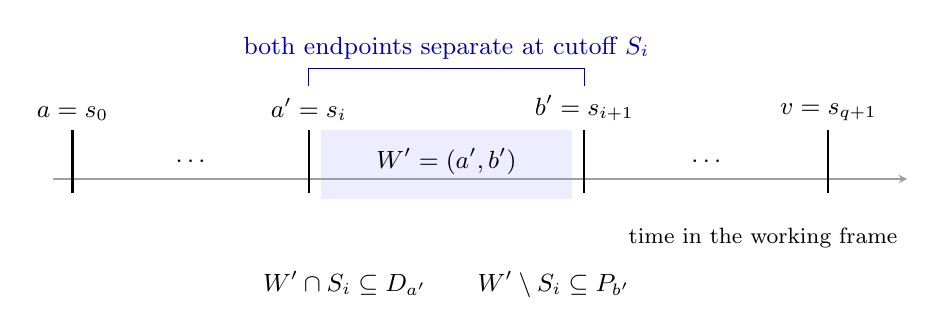
\begin{tikzpicture}[x=1cm,y=1cm,font=\small,>=stealth]
  \fill[blue!7] (3.15,-.25) rectangle (6.35,.62);
  \draw[->,gray!75] (-.25,0) -- (10.6,0);
  \node[anchor=east,font=\footnotesize] at (10.6,-.75)
    {time in the working frame};
  \foreach \x in {0,3,6.5,9.6}
    {\draw[thick] (\x,-.18) -- (\x,.62);}
  \node[above] at (0,.62) {$a=s_0$};
  \node[above] at (3,.62) {$a'=s_i$};
  \node[above] at (6.5,.62) {$b'=s_{i+1}$};
  \node[above] at (9.6,.62) {$v=s_{q+1}$};
  \node at (4.75,.22) {$W'=(a',b')$};
  \node at (1.5,.22) {$\cdots$};
  \node at (8.05,.22) {$\cdots$};
  \draw[blue!65!black] (3,1.18) -- (3,1.4) -- (6.5,1.4) -- (6.5,1.18);
  \node[above,text=blue!65!black] at (4.75,1.4)
    {both endpoints separate at cutoff $S_i$};
  \node[anchor=north,align=center] at (4.75,-1.05)
    {$W'\cap S_i\subseteq D_{a'}$\qquad
     $W'\setminus S_i\subseteq P_{b'}$};
\end{tikzpicture}

\caption{One side of a node, viewed in its working frame.
Each nonempty gap uses the cutoff belonging to its strict walk step.
The endpoints separate that same cutoff, although adjacent gaps may
use different cutoffs. The horizontal arrow denotes schedule time,
not a precedence relation.}
\label{fig:shared-cutoff}
\end{figure}

It remains to give each child a short list selecting exactly
its high jobs, and to preserve the global boundary invariants.
The following sections prove these claims by a top-down induction.
When a child of \(W\) is constructed, all data for \(W\) and its
ancestors have already been constructed. No claim about a deeper
descendant is used.

\begin{table}[t]
\centering
\small
\begin{tabular}{@{}p{.25\textwidth}p{.69\textwidth}@{}}
\toprule
Proof component & Interface used by the next step \\
\midrule
Shared cutoffs & A normalized side, a starting separator, and successive
priority prefixes give two boundaries separating the same cutoff
(\Cref{lem:shared}). \\[4pt]
Child intervals & A valid parent gives a center and strictly smaller gaps
with their shared cutoffs (\Cref{lem:edge-labels}). \\[4pt]
Global lists & Each child receives its high-job set and first invariant
through at most five upset entries, each with fewer than \(40\) leaves
(\Cref{lem:update-labels,lem:list-length,lem:entry-size}). \\[4pt]
Boundary stability & Parent invariants and side normalization give child
Invariants~\ref{inv:past}--\ref{inv:swap}, including all future feasible
child reorderings (\Cref{lem:past,lem:swap}). \\[4pt]
Finite descriptions & Valid lists and boundaries give global child sets
and relative splits with fewer than \(500\) leaves
(\Cref{lem:global-child,lem:relative-splits,lem:final-count}). \\
\bottomrule
\end{tabular}
\caption{The contracts connecting the structural proof. The executable
dynamic program consumes the final node sets and split sets; lists and
normalized schedules are used to prove that these sets suffice.}
\label{tab:contracts}
\end{table}
